\documentclass[11pt]{scrartcl}
\usepackage[utf8]{inputenc}
\usepackage{mathtools}
\usepackage{amssymb}
\usepackage{listings}
\usepackage{bm}
\usepackage{graphicx}
\usepackage{qtree}
\lstset
{ %Formatting for code in appendix
	language=Matlab,
	basicstyle=\footnotesize,
	numbers=left,
	stepnumber=1,
	showstringspaces=false,
	tabsize=1,
	breaklines=true,
	breakatwhitespace=false,
}
\begin{document}
\centerline{\LARGE{\textbf{CSE881 HW3}}}
\centerline{\large{\textit{Nan Cao,\  A52871775}}}
\centerline{\large{\textit{Sep 25th, 2016}}}
% \maketitle
\section*{Problem 1}
\textbf{(a)}\\
\begin{equation*}
\begin{aligned}
d(\bm{x},\bm{y})&=1-c(\bm{x},\bm{y})\\
c(\bm{x},\bm{y})&=1-d(\bm{x},\bm{y})\\
cos(\bm{x},\bm{y})&=1-d(\bm{x},\bm{y})\\
cos \frac{\pi}{4}  &\leq cos(s,y) \leq cos 0\\
1- cos 0  &\leq d(\bm{x},\bm{y}) \leq cos 1-\frac{\pi}{4}\\
0  &\leq d(\bm{x},\bm{y}) \leq 1\\
\end{aligned}
\end{equation*}
\\
\textbf{(b)}\\
Based on (a), Yes, it satisfies the positivity preperty\\
\\
\textbf{(c)}\\
\begin{equation*}
\begin{aligned}
d(\bm{x},\bm{y})&=1-cos(\bm{x},\bm{y})\\
&=1-cos(\bm{y},\bm{x})\\
&=d(\bm{y},\bm{x})\\
\end{aligned}
\end{equation*}
 Yes, it satisfies the symmetry preperty\\
 \\
 \textbf{(d)}\\
 No, for example:
\begin{equation*}
\begin{aligned}
\bm{x}&=(3,4)\\
\bm{y}&=(5,12)\\
\bm{z}&=(7,24)\\
d(\bm{x},\bm{y})&=1-\frac{15+48}{5*13}=\frac{2}{65}\\
d(\bm{y},\bm{z})&=1-\frac{35+288}{13*25}=\frac{2}{325}\\
d(\bm{x},\bm{z})&=1-\frac{21+96}{5*25}=\frac{8}{125}\\
d(\bm{x},\bm{y})+d(\bm{y},\bm{z})&=\frac{12}{325}<\frac{8}{125}=d(\bm{x},\bm{z})\\
\end{aligned}
\end{equation*}
\section*{Problem 2}
\textbf{(a)}\\
Let\ $ \bm{U}(\bm{q},\epsilon)$\ denote a circle neighbourhood of point\ $ \bm{q}$ within a radius of  $\epsilon$;\\
\begin{equation*}
\begin{aligned}
\forall \bm{p}&\in \bm{S}\\
% \end{aligned}
% \end{equation*}
% i)\\
% \begin{equation*}
% \begin{aligned}
\\
d(\bm{p},\bm{y})+d(\bm{p},\bm{q})&\geq d(\bm{q},\bm{y})\\
d(\bm{p},\bm{q})& \geq d(\bm{q},\bm{y})-d(\bm{p},\bm{y})\\
% \end{aligned}
% \end{equation*}
% ii)\\
% \begin{equation*}
% \begin{aligned}
d(\bm{q},\bm{y})+d(\bm{p},\bm{q})&\geq d(\bm{p},\bm{y})\\
d(\bm{p},\bm{q})&\geq d(\bm{p},\bm{y})-d(\bm{q},\bm{y})\\
if \ min[d(\bm{q},\bm{y})-d(\bm{p},\bm{y})&, d(\bm{p},\bm{y}-d(\bm{q},\bm{y})] >\epsilon\\
d(\bm{p},\bm{q})&>\epsilon\\
\bm{p} &\notin \bm{U}(\bm{q},\epsilon)\\
No\ more\ calculation\ needed.\\
\\
d(\bm{p},\bm{q})&\leq d(\bm{p},\bm{y})+d(\bm{q},\bm{y})\\
 if \ d(\bm{p},\bm{y})+d(\bm{q},\bm{y})&< \epsilon\\
d(\bm{p},\bm{q})& < \epsilon\\
\bm{p} &\in \bm{U}(\bm{q},\epsilon)\\
No\ more\ calculation\ needed.\\
\end{aligned}
\end{equation*}
\\
\textbf{(b)}\\
Let\ $ \bm{U}(\bm{x},\beta)$\ denote a circle neighbourhood of point\ $ \bm{x}$ within a radius of  $\beta$;\\
\begin{equation*}
\begin{aligned}
\forall \bm{x_i}&\in \bm{S};\\
we\ have \ \bm{x_i^*}&\in \bm{\Psi}\ (i\in\mathbb{N}^*)\\
d(\bm{x_i},\bm{x_i}^*) &\leq \epsilon\\
\forall i,j&\in\mathbb{N}^*\\
% if\ d(\bm{x_i^*},{x_j^*})&\leq \epsilon\\
\\
d(\bm{x_i},\bm{x_j})&\leq d(\bm{x_i},\bm{x_i^*})+d(\bm{x_i^*},\bm{x_j})\\
&\leq d(\bm{x_i},\bm{x_i^*})+(d(\bm{x_i^*},\bm{x_j^*})+d(\bm{x_j},\bm{x_j^*})\\
&=(d(\bm{x_i},\bm{x_i^*})+d(\bm{x_j},\bm{x_j^*}))+d(\bm{x_i^*},\bm{x_j^*})\\
&\leq 2\epsilon+d(\bm{x_i^*},\bm{x_j^*})\\
if\ 2\epsilon+d(\bm{x_i^*},\bm{x_j^*})&< \beta\\
d(\bm{x_i},\bm{x_j})&< \beta\\
\bm{x_i} &\in \bm{U}(\bm{x_j},\beta)\\
No\ more\ calculation\ needed.\\
\\
d(\bm{x_i^*},\bm{x_j}^*)&\leq d(\bm{x_i},\bm{x_i^*})+d(\bm{x_i},\bm{x_j^*})\\
&\leq d(\bm{x_i},\bm{x_i^*})+(d(\bm{x_i},\bm{x_j})+d(\bm{x_j},\bm{x_j^*})\\
&=(d(\bm{x_i},\bm{x_i^*})+d(\bm{x_j},\bm{x_j^*}))+d(\bm{x_i},\bm{x_j})\\
&\leq 2\epsilon+d(\bm{x_i},\bm{x_j})\\
d(\bm{x_i},\bm{x_j})&\geq d(\bm{x_i^*},\bm{x_j}^*)-2\epsilon\\
if\  d(\bm{x_i^*},\bm{x_j}^*)-2\epsilon &> \beta\\
d(\bm{x_i},\bm{x_j})&> \beta\\
\bm{x_i} &\notin \bm{U}(\bm{x_j},\beta)\\
No\ more\ calculation\ needed.\\
\end{aligned}
\end{equation*}
\\
\section*{Problem 3}
 \textbf{(a)}\\
\begin{equation*}
\begin{aligned}
Var(\bm{x})&=0.07263963\\
Var(\bm{y})&=0.1110305\\
\end{aligned}
\end{equation*}
The variance on dimension $\bm{y}$ is larger.The median of this dimension is 0.5472\\
\\
For the first part:\\
\begin{equation*}
\begin{aligned}
var(0.5853 0.2238 0.5060 0.7513)&=0.04854933\\
var( 0.1386 0.1493 0.2543 0.2575)&=0.004198389\\
\end{aligned}
\end{equation*}
The variance on dimension $\bm{x}$ is larger. The median is 0.5060.\\
\\
For the second part:\\
\begin{equation*}
\begin{aligned}
var(0.1190 0.2551 0.4984 0.9597)&=0.1364748\\
var(0.6991 0.8407 0.8909 0.9593)&=0.01215053\\
\end{aligned}
\end{equation*}
The variance on dimension $\bm{x}$ is larger. The median is 0.2551.\\
\\
For ( 0.5853,0.1386),( 0.7513 ,0.2575):
\begin{equation*}
\begin{aligned}
var(0.5853,0.7513)&=0.013778\\
var(0.1386 ,0.2575)&=0.007068605\\
\end{aligned}
\end{equation*}
The variance on dimension $\bm{x}$ is larger. The median is 0.5853.\\
\\
For  (0.4984,0.8909),(0.9597,0.9593)
\begin{equation*}
\begin{aligned}
var(0.4984,0.9597)&=0.1063988\\
var(0.8909,0.9593)&=0.00233928\\
\end{aligned}
\end{equation*}
The variance on dimension $\bm{x}$ is larger. The median is 0.4984\\
\\
The ordered date set:
\begin{equation*}
\begin{aligned}
\begin{matrix}
                    &     [x]               &           [y]         \\
 [1,]            &     0.2238       &           0.1493 \\
 [2,]            &     0.5060       &           0.2543 \\
 [3,]            &     0.5853       &           0.1386 \\
 [4,]            &     0.7513       &           0.2575 \\
 [5,]            &     0.3404       &           0.5472\\
 [6,]            &     0.1190       &           0.6991 \\
 [7,]            &     0.2551       &           0.8407\\
 [8,]            &     0.4984       &           0.8909 \\
 [9,]            &     0.9597       &           0.9593 \\
\end{matrix}
\end{aligned}
\end{equation*}
\\
\\
\Tree[.(0.3404,0.5472) 
	[.(0.5060,0.2543)
		[.(0.2238,0.1493) ]
                 	[.(0.5853,0.1386) (0.7513,0.2575)  ]
                 ]
                 [.(0.2551,0.8407) 
                  	[.(0.1190,0.6991) ]
                 	[.(0.4984,0.8909) (0.9597,0.9593)  ]
                  ]
          ]
 \\
 \textbf{(b)}\\
 \begin{figure} 
	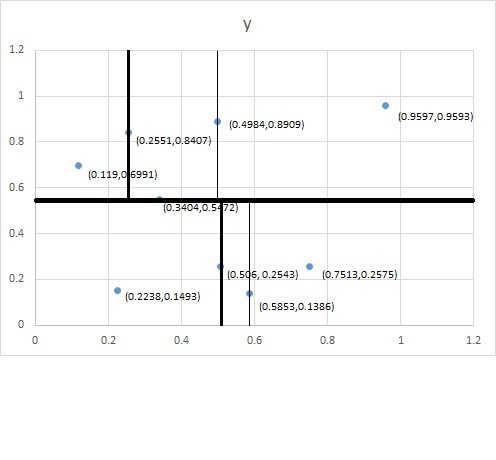
\includegraphics[width=5.5in,height=5.5in]{Q3.jpg}
	\caption{Problem 3 (b)}
\end{figure}
\\
 \textbf{(c)}\\
  \begin{equation*}
\begin{aligned}
 (0.3404,0.5472)\\
 (0.2551,0.8407) \\
 (0.2238,0.1493)\\
 (0.5853,0.1386)\\
 (0.4984,0.8909)\\
 \end{aligned}
\end{equation*}
 \\
 \section*{Problem 4}
 \textbf{(a)}
 \begin{equation*}
\begin{aligned}
\begin{pmatrix}
&d_1&d_2&d_3&d_4\\
d_1 & 1 &\frac{1}{3} & \frac{2}{7}&\frac{3}{8}\\
d_2 & \frac{1}{3} & 1 & \frac{3}{7}&\frac{5}{7}\\
d_3 & \frac{2}{7} &\frac{3}{7}&1&\frac{1}{7}\\
d_4 &\frac{3}{8} &\frac{5}{7}&\frac{1}{7}& 1\\
\end{pmatrix}
\end{aligned}
\end{equation*}
\textbf{(b)}\\
Calculation for this question are shown at the end of the work.
 \begin{equation*}
\begin{aligned}
\begin{pmatrix}
         &   h_1&   h_2   &h_3   &h_4  & h_5& h_6 \\
d_1 &   10   &   3        &   2     &   3     &   9   &   10 \\
d_2 &   10   &   3        &   4     &   6     &   6   &   10 \\
d_3 &   3     &   3        &   4      &   4     &   4   &   4   \\
d_4 &   10   &   7        &   2     &   6      &   6   &   10 \\
\end{pmatrix}
\end{aligned}
\end{equation*}
\\
\textbf{(c)}
 \begin{equation*}
\begin{aligned}
\begin{pmatrix}
          & d_1              & d_2             & d_3             & d_4\\
d_1  & 1                  &\frac{1}{2} &\frac{1}{6} &\frac{1}{2}\\
d_2  &\frac{1}{2} &1                    &\frac{1}{3} &\frac{2}{3}\\
d_3  &\frac{1}{6} &\frac{1}{3} &1                    &0\\
d_4  &\frac{1}{2} &\frac{2}{3} &0                   &1\\
\end{pmatrix}
\end{aligned}
\end{equation*}
\textbf{(d)}
Yes, it's $p[h(d_2)=h(d_4)]$\\
\\
\textbf{(e)}
Yes, it's $p[h(d_3)=h(d_4)]$\\
\\
\section*{Calculation for 3(b)}

\begin{equation*}
\begin{aligned}
\begin{pmatrix}
\bm{[10]} & \bm{[3]} & \bm{[8]} & \bm{[9]} & \bm{[6]} & \bm{[5]} & \bm{[4]} & \bm{[2]} & \bm{[1]} & \bm{[7]}\\
1   &   1   &   0   &   1   &   0   &   0   &   0   &   1   &   1   &    1\\
1   &   1   &   1   &   0   &   1   &   0   &   1   &   1   &   0   &    1\\
0   &   1   &   0   &   0   &   0   &   0   &   1   &   0   &   0   &    1\\
1   &   0   &   1   &   0   &   1   &   0   &   0   &   1   &   0   &    1\\
\end{pmatrix}\\
h(D_1)=(10,10,3,10)\\
\\
\begin{pmatrix}
\bm{[3]} & \bm{[9]} & \bm{[7]} & \bm{[5]} & \bm{[4]} & \bm{[2]} & \bm{[6]} & \bm{[8]} & \bm{[1]} & \bm{[10]}\\
1   &   1   &   1   &   0   &   0   &   1   &   0   &   0   &   1   &    1\\
1   &   0   &   1   &   0   &   1   &   1   &   1   &   1   &   0   &    1\\
1   &   0   &   1   &   0   &   1   &   0   &   0   &   0   &   0   &    0\\
0   &   0   &   1   &   0   &   0   &   1   &   1   &   1   &   0   &    1\\
\end{pmatrix}\\
h(D_2)=(3,3,3,7)\\
\\
\begin{pmatrix}
\bm{[4]} & \bm{[2]} & \bm{[3]} & \bm{[1]} & \bm{[7]} & \bm{[5]} & \bm{[6]} & \bm{[9]} & \bm{[8]} & \bm{[10]}\\
0   &   1   &   1   &   1   &   1   &   0   &   0   &   1   &   0   &    1\\
1   &   1   &   1   &   0   &   1   &   0   &   1   &   0   &   1   &    1\\
1   &   0   &   1   &   0   &   1   &   0   &   0   &   0   &   0   &    0\\
0   &   1   &   0   &   0   &   1   &   0   &   1   &   0   &   1   &    1\\
\end{pmatrix}\\
h(D_3)=(2,4,4,2)\\
\\
\begin{pmatrix}
\bm{[6]} & \bm{[4]} & \bm{[3]} & \bm{[10]} & \bm{[7]} & \bm{[8]} & \bm{[5]} & \bm{[9]} & \bm{[1]} & \bm{[2]}\\
0   &   0   &   1   &   1   &   1   &   0   &   0   &   1   &   1   &    1\\
1   &   1   &   1   &   1   &   1   &   1   &   0   &   0   &   0   &    1\\
0   &   1   &   1   &   0   &   1   &   0   &   0   &   0   &   0   &    0\\
1   &   0   &   0   &   1   &   1   &   1   &   0   &   0   &   0   &    1\\
\end{pmatrix}\\
h(D_4)=(3,6,4,6)\\
\\
\begin{pmatrix}
\bm{[9]} & \bm{[6]} & \bm{[8]} & \bm{[5]} & \bm{[1]} & \bm{[4]} & \bm{[7]} & \bm{[2]} & \bm{[3]} & \bm{[10]}\\
1   &   0   &   0   &   0   &   1   &   0   &   1   &   1   &   1   &    1\\
0   &   1   &   1   &   0   &   0   &   1   &   1   &   1   &   1   &    1\\
0   &   0   &   0   &   0   &   0   &   1   &   1   &   0   &   1   &    0\\
0   &   1   &   1   &   0   &   0   &   0   &   1   &   1   &   0   &    1\\
\end{pmatrix}\\
h(D_5)=(9,6,4,60)\\
\\
\begin{pmatrix}
\bm{[10]} & \bm{[1]} & \bm{[4]} & \bm{[6]} & \bm{[9]} & \bm{[2]} & \bm{[7]} & \bm{[3]} & \bm{[8]} & \bm{[5]}\\
1   &   1   &   0   &   0   &   1   &   1   &   1   &   1   &   0   &    0\\
1   &   0   &   1   &   1   &   0   &   1   &   1   &   1   &   1   &    0\\
0   &   0   &   1   &   0   &   0   &   0   &   1   &   1   &   0   &    0\\
1   &   0   &   0   &   1   &   0   &   1   &   1   &   0   &   1   &    0\\
\end{pmatrix}\\
h(D_6)=(10,10,4,10)\\
\\
\end{aligned}
\end{equation*}
\end{document}
% \begin{equation*}
% \begin{aligned}
% \end{aligned}
% \end{equation*}